%convolution result
\par \indent The convolution process returns three haemodynamic response 
predictions corresponding to neural conditions for parametric gain, parametric 
loss, and distance from indifference respectively, that are shown in the 
figures below [Figure \ref{fig:convolution}]. These haemodynamic responses are 
crucial to fMRI analysis because fMRI measures haemodynamic responses of the 
brain to locate neural activities regions. 

\begin{figure}[h!]
\centering
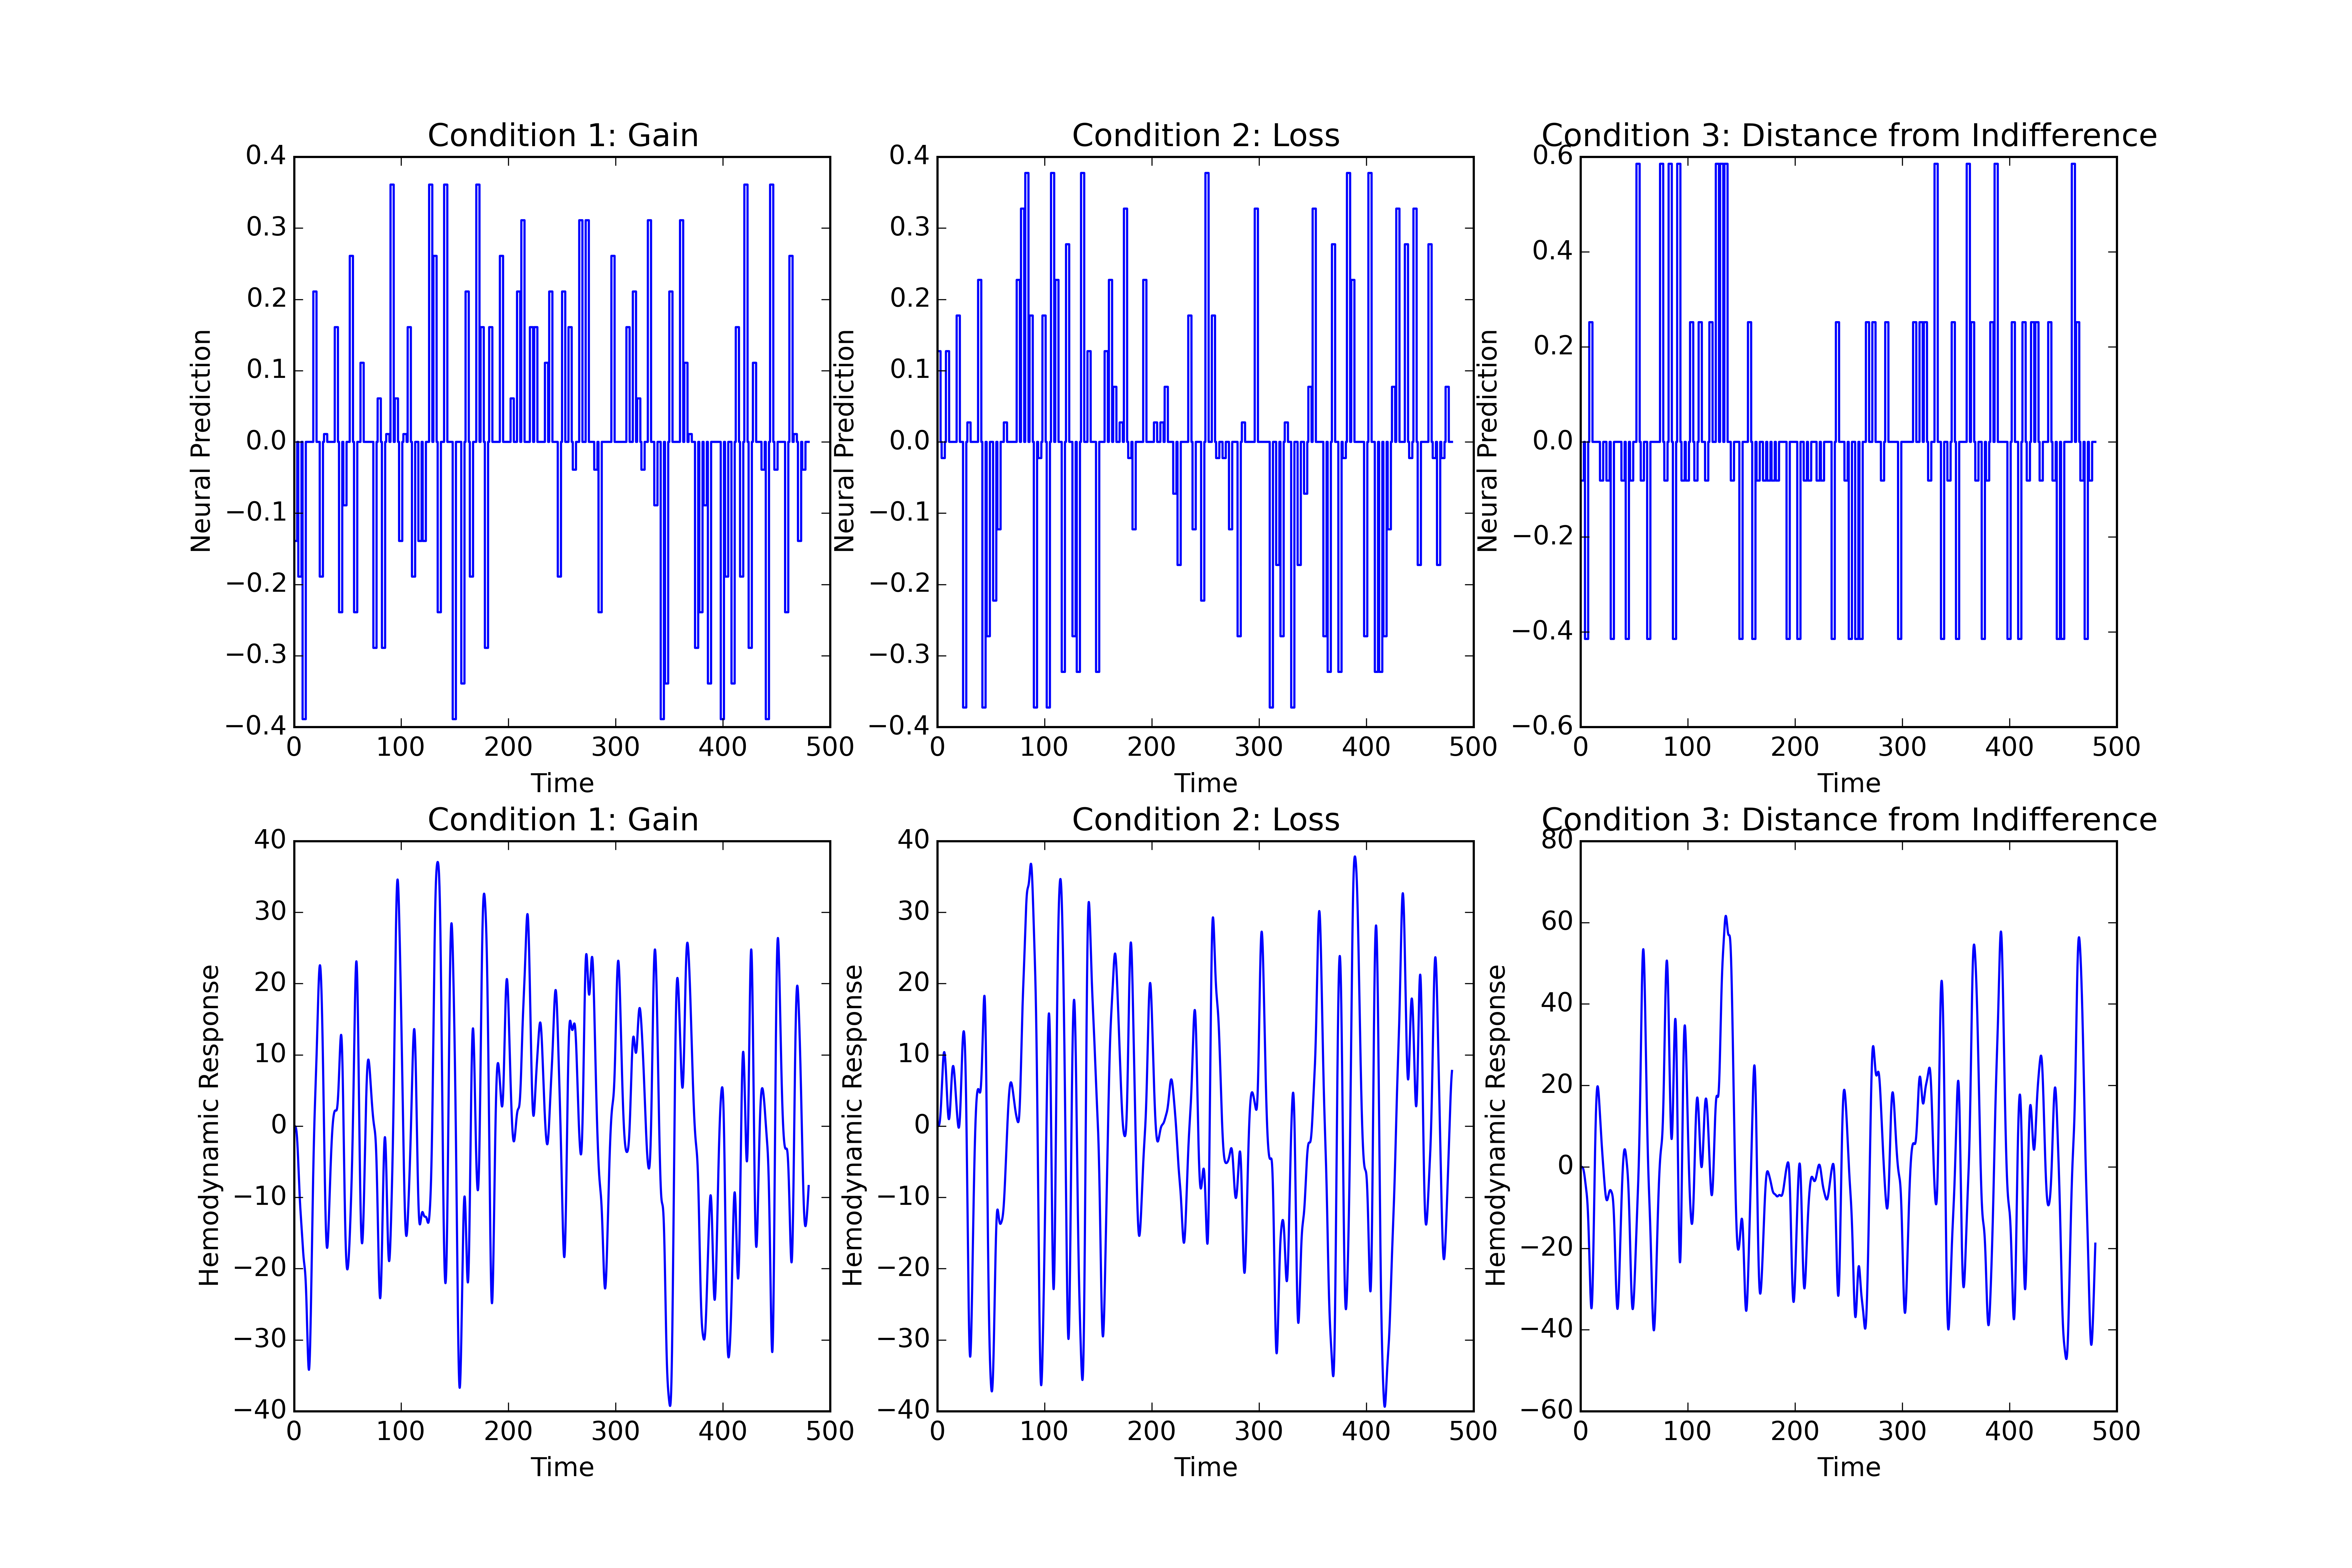
\includegraphics[width=120mm]{images/convolution3cond.png}
\caption{Neural and Haemodynamic Response Predictions for Three Conditions for Subject 1 in Run 1}
\label{fig:convolution}
\end{figure}
